\chapter{Metodologie și Experimente}
\label{cap:metodologie}

\section{Formularea Problemei}
\label{sec:formulare}

Problema abordată în această lucrare nu se încadrează în tiparul clasic
al predicției pre-meci, în care un model estimează rezultatul unui meci
înainte ca acesta să înceapă, pe baza statisticilor istorice ale echipelor.
În schimb, sistemul propus operează \textit{eveniment cu eveniment},
reconstituind evoluția probabilistică a unui meci deja încheiat pe baza
acțiunilor înregistrate în cursul partidei.

Intrarea modelului este o reprezentare instantanee (\textit{snapshot}) a
stării meciului la un moment dat $t$, codificată ca un vector de
caracteristici $\mathbf{x}_t \in \mathbb{R}^{33}$, unde $33$ este numărul
total de caracteristici utilizate de modelul final. Acest vector
sintetizează informațiile disponibile până la momentul $t$: scorul curent,
expected goals (golurile așteptate, prescurtat xG în literatura de
specialitate) acumulate de fiecare echipă, numărul de șuturi și de pase,
presiunea exercitată, cartonașele primite, precum și un set de
caracteristici derivate care surprind dinamica recentă a jocului
(momentum, context temporal și context de joc). Formal, structura
vectorului este:

\begin{equation}
    \mathbf{x}_t = \bigl[
        \text{score\_diff}_t,\;
        \text{xg\_diff}_t,\;
        \text{shots\_home}_t,\;
        \text{shots\_away}_t,\;
        \text{minute}_t,\;
        \text{pressure}_t,\;
        \ldots
    \bigr] \in \mathbb{R}^{33}
\end{equation}

unde $\text{score\_diff}_t$ este diferența de scor la momentul $t$,
$\text{xg\_diff}_t$ este diferența de expected goals, $\text{shots\_home}_t$
și $\text{shots\_away}_t$ sunt numărul cumulat de șuturi ale fiecărei
echipe, $\text{minute}_t$ este minutul de joc, iar $\text{pressure}_t$
reprezintă presiunea exercitată. Lista completă a celor 33 de
caracteristici este detaliată în Secțiunea~\ref{sec:feature_engineering}.

Un snapshot nu corespunde unui interval fix de timp, deoarece datele
StatsBomb sunt înregistrate la nivel de eveniment, nu la intervale
regulate. În consecință, într-un minut de joc pot exista zeci de snapshots
(atunci când există multe acțiuni) sau doar câteva (atunci când jocul este
lent). Fiecare eveniment din meci, fie o pasă, un șut sau o faultare,
generează un nou snapshot prin actualizarea cumulativă a statisticilor.

Ieșirea modelului este o distribuție de probabilitate peste cele trei
rezultate posibile ale meciului: victoria gazdelor (Home Win), egalul
(Draw) și victoria oaspeților (Away Win):

\begin{equation}
    \hat{\mathbf{p}}_t = \bigl(
        P(\text{Home Win} \mid \mathbf{x}_t),\;
        P(\text{Draw} \mid \mathbf{x}_t),\;
        P(\text{Away Win} \mid \mathbf{x}_t)
    \bigr), \quad \sum_{k=1}^{3} \hat{p}_{t,k} = 1
\end{equation}

unde $P(\cdot \mid \mathbf{x}_t)$ reprezintă probabilitatea condiționată a
fiecărui rezultat dat fiind vectorul de caracteristici $\mathbf{x}_t$, iar
constrângerea $\sum_{k=1}^{3} \hat{p}_{t,k} = 1$ garantează că cele trei
probabilități formează o distribuție validă. Această distribuție este
estimată de model la fiecare moment $t$ al meciului, producând o
\textit{traiectorie probabilistică} pe durata întregii partide.
Figura~\ref{fig:win_prob_example} ilustrează un exemplu tipic al acestei
traiectorii pentru un meci din setul de date.

\begin{figure}[H]
    \centering
    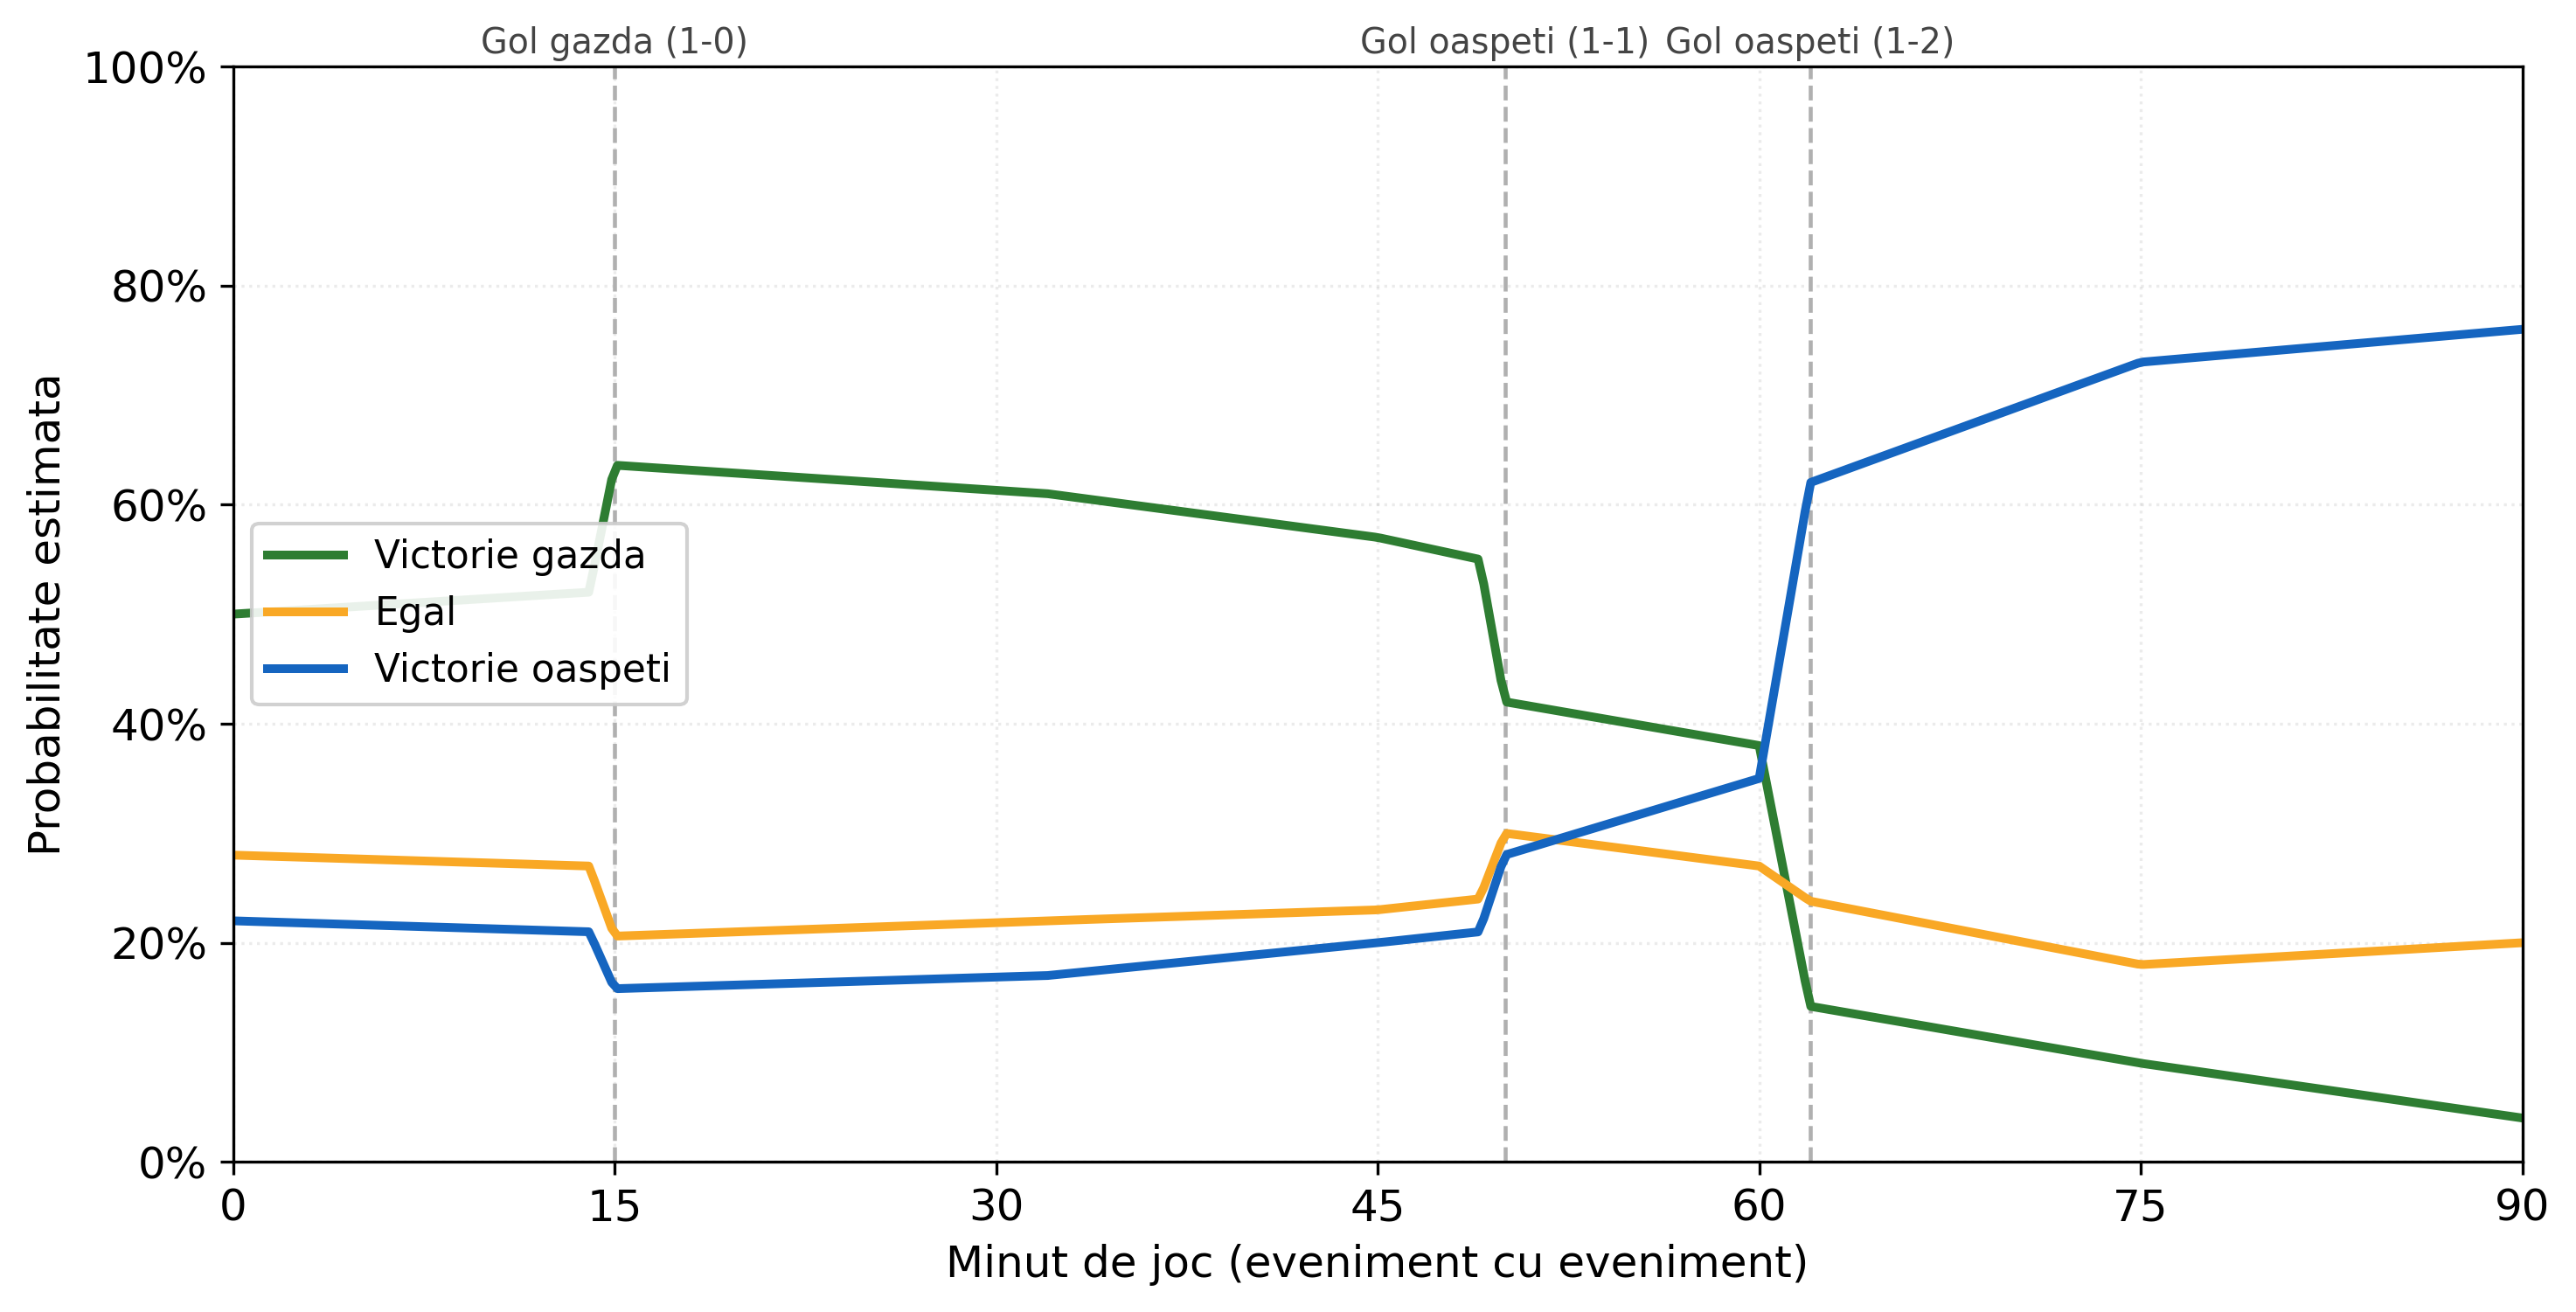
\includegraphics[width=0.88\textwidth]{figures/win_prob_trajectory.png}
    \caption{Exemplu de traiectorie probabilistică generată de model
    pentru un meci din setul de date. Fiecare punct de pe axa
    orizontală corespunde unui eveniment înregistrat, iar variațiile
    bruște corespund golurilor și cartonașelor roșii.}
    \label{fig:win_prob_example}
\end{figure}

Problema este formulată ca o clasificare multi-clasă la nivel de
eveniment: fiecare snapshot $\mathbf{x}_t$ este etichetat cu rezultatul
final al meciului din care provine ($y \in \{0, 1, 2\}$, corespunzând
victoriei oaspeților, egalului și victoriei gazdelor). Modelul învață
astfel să asocieze starea curentă a jocului cu probabilitatea ca fiecare
rezultat să se materializeze la finalul partidei.

Trebuie subliniat că aceasta este o abordare \textbf{post-meci}: modelul
nu are acces la informații viitoare față de momentul $t$, însă întregul
pipeline este rulat după încheierea meciului, pe baza evenimentelor deja
înregistrate. Arhitectura este proiectată deliberat pentru a permite
extensia naturală către predicția în timp real, fără modificări
structurale; singura diferență ar consta în faptul că evenimentele ar fi
furnizate într-un flux live, în loc să fie citite dintr-un fișier static.

% ----------------------------------------------------------------
\section{Setul de date}

Experimentele au fost realizate pe datele publice StatsBomb Open Data
\cite{StatsBomb}, care conțin \textbf{12.188.949 de evenimente} provenite
din \textbf{3.464 de meciuri}, acoperind competițiile majore europene
(Premier League, La Liga, Serie A, Bundesliga, Ligue 1) din perioada
2017--2023. În format brut (JSON) setul ocupă aproximativ 2.8 GB; după
preprocesare și agregare la nivel de eveniment rezultă un set tabular de
aproximativ 1.87 GB în format CSV, utilizat efectiv la antrenare. Fiecare
eveniment include 24 de caracteristici de bază de înaltă calitate,
descrise în Secțiunea~\ref{sec:feature_engineering}.

Raportat la cele 3.464 de meciuri, rezultă o medie de aproximativ
\textbf{3.519 de evenimente per meci} (mediană de 3.503, cu valori între
2.101 și 5.190 de evenimente pe meci), ceea ce confirmă granularitatea
ridicată a datelor StatsBomb și justifică abordarea la nivel de eveniment:
fiecare partidă furnizează câteva mii de snapshots din care modelul poate
învăța dinamica probabilistică. Variația numărului de evenimente între
meciuri reflectă ritmul diferit al partidelor, dat de numărul de pase,
șuturi și acțiuni de presing înregistrate.

La nivelul rezultatelor finale, distribuția celor 3.464 de meciuri pe cele
trei clase este dezechilibrată, reflectând avantajul terenului propriu
documentat în literatura sportivă \cite{Robberechts2019}: victoriile
gazdelor reprezintă 45.2\% din meciuri (1.565 de partide), victoriile
oaspeților 31.8\% (1.102 partide), iar egalurile 23.0\% (797 de partide).
Tabelul~\ref{tab:distributie_clase} sintetizează această distribuție.
Dezechilibrul natural al claselor, în care egalurile sunt clar
minoritare, a fost luat în considerare la configurarea hiperparametrului
\texttt{class\_weight} în etapa de optimizare.

\begin{table}[htbp]
\centering
\begin{tabular}{|l|r|r|}
\hline
\textbf{Rezultat final} & \textbf{Număr meciuri} & \textbf{Pondere} \\
\hline
Victorie gazde (Home Win) & 1.565 & 45.2\% \\
\hline
Victorie oaspeți (Away Win) & 1.102 & 31.8\% \\
\hline
Egal (Draw) & 797 & 23.0\% \\
\hline
\textbf{Total} & \textbf{3.464} & \textbf{100\%} \\
\hline
\end{tabular}
\caption{Distribuția celor 3.464 de meciuri pe cele trei clase de rezultat
         final, la nivelul întregului set de date StatsBomb.}
\label{tab:distributie_clase}
\end{table}

% ----------------------------------------------------------------
\section{Reprezentarea datelor și construirea caracteristicilor}
\label{sec:feature_engineering}

Înainte de începerea experimentării, au fost analizate lucrările existente
din literatură, în special modelul propus de Robberechts et al.
\cite{Robberechts2019}, care sugerează că performanța modelelor de
predicție poate fi îmbunătățită prin captarea dinamicii temporale a
jocului. Pe baza acestei idei, au fost construite \textbf{33 de
caracteristici in-game}, organizate în două categorii principale:
caracteristici de bază și caracteristici derivate.

\subsection{Caracteristici de bază}

Caracteristicile de bază descriu starea instantanee a meciului la fiecare
moment de timp și constituie fundamentul informațional al modelului. Cele
24 de caracteristici de bază sunt grupate în șase categorii, prezentate în
Tabelul~\ref{tab:features_baza}.

\begin{table}[h!]
\centering
\begin{tabular}{ll}
\hline
\textbf{Categorie} & \textbf{Caracteristici} \\
\hline
Temporal & \texttt{minute}, \texttt{timestamp\_seconds} \\
Scor & \texttt{score\_home}, \texttt{score\_away}, \texttt{score\_diff} \\
Expected goals & \texttt{xg\_home}, \texttt{xg\_away}, \texttt{xg\_diff} \\
Șuturi & \texttt{shots\_home}, \texttt{shots\_away}, \\
       & \texttt{shots\_on\_target\_home}, \texttt{shots\_on\_target\_away} \\
Pase & \texttt{passes\_home}, \texttt{passes\_away} \\
Cartonașe & \texttt{yellow\_cards\_home}, \texttt{yellow\_cards\_away}, \\
          & \texttt{red\_cards\_home}, \texttt{red\_cards\_away},
            \texttt{cards\_diff} \\
Presiune și context & \texttt{pressure\_home}, \texttt{pressure\_away}, \\
                    & \texttt{under\_pressure}, \texttt{counterpress},
                      \texttt{is\_home\_team} \\
\hline
\end{tabular}
\caption{Cele 24 de caracteristici de bază utilizate în antrenare,
         grupate pe categorii.}
\label{tab:features_baza}
\end{table}

Pentru a permite reproducerea rezultatelor și interpretarea corectă a
modelului, fiecare categorie de caracteristici merită o descriere a
formatului și a intervalului de valori. Caracteristicile temporale
\texttt{minute} (minutul de joc, valoare întreagă de la 0 la peste 90,
incluzând prelungirile) și \texttt{timestamp\_seconds} (timpul scurs în
secunde) localizează snapshot-ul în desfășurarea partidei. Caracteristicile
de scor \texttt{score\_home} și \texttt{score\_away} rețin numărul de goluri
marcate de fiecare echipă până la momentul curent (valori întregi
nenegative), iar \texttt{score\_diff} este diferența dintre ele, pozitivă
când gazdele conduc și negativă în caz contrar. Caracteristicile de
expected goals \texttt{xg\_home} și \texttt{xg\_away} sunt valori continue
nenegative care cumulează calitatea ocaziilor fiecărei echipe (fiecare șut
contribuie cu o probabilitate de marcare între 0 și 1), iar
\texttt{xg\_diff} măsoară superioritatea ofensivă cumulată.
Caracteristicile de șuturi și pase sunt contoare cumulate (valori întregi
nenegative) care cresc monoton pe parcursul meciului. Cartonașele sunt de
asemenea contoare cumulate per echipă, iar \texttt{cards\_diff} reflectă
diferența de disciplină dintre echipe.

Caracteristicile de presiune sunt derivate din tipurile de evenimente
StatsBomb: \texttt{pressure\_home} și \texttt{pressure\_away} contorizează
acțiunile de presing înregistrate pentru fiecare echipă, \texttt{under\_pressure}
indică acțiunile efectuate sub presiunea adversarului, iar
\texttt{counterpress} numără acțiunile de contrapresing imediat după
pierderea posesiei. În sfârșit, \texttt{is\_home\_team} este un indicator
binary (0 sau 1) care marchează perspectiva din care este construit
snapshot-ul.

\subsection{Caracteristici derivate}

Inspirate din literatura de specialitate, caracteristicile derivate au fost
introduse pentru a surprinde dinamica temporală a meciului, informație pe
care caracteristicile de bază nu o pot reprezenta în mod direct. Cele 9
caracteristici adăugate sunt organizate în trei categorii: momentum,
context temporal și context de joc.

Categoria de \textit{momentum} surprinde tendințele recente ale jocului
prin variații calculate pe ferestre scurte de timp. Caracteristica
\texttt{score\_momentum} reprezintă variația scorului între evenimente
consecutive, capturând schimbările recente ale avantajului unei echipe.
Caracteristica \texttt{xg\_momentum} măsoară evoluția expected goals pe o
fereastră mobilă de trei evenimente, reflectând tendințele ofensive
recente, iar \texttt{pressure\_momentum} cuantifică, analog, variația
presiunii exercitate de echipe în ultimele momente ale jocului.

Categoria de \textit{context temporal} codifică faza meciului în care se
află un eveniment. Caracteristica \texttt{time\_remaining\_norm} reprezintă
timpul rămas până la finalul partidei, normalizat în intervalul $[0, 1]$
prin raportare la minutul maxim al meciului respectiv (ceea ce tratează
corect prelungirile). Indicatorii binari \texttt{is\_early\_game} și
\texttt{is\_late\_game} marchează, respectiv, primele 30 de minute
(minutul mai mic de 30) și ultimele faze ale meciului (minutul mai mare de
75), iar \texttt{is\_crunch\_time} indică momentele echilibrate, definite
ca situațiile în care diferența de scor în valoare absolută este cel mult
egală cu 1.

Categoria de \textit{context de joc} adaugă informații despre poziția
echipelor în partidă. Caracteristica \texttt{is\_winning} este un indicator
binary care arată dacă echipa gazdă se află în avantaj la momentul
respectiv (diferență de scor strict pozitivă), iar \texttt{score\_xg\_gap}
măsoară diferența dintre scorul real la momentul curent și expected goals
acumulate, fiind utilizată pentru a estima eficiența ofensivă: o valoare
pozitivă indică o echipă care a marcat mai mult decât sugerează calitatea
ocaziilor, iar o valoare negativă indică ineficiență ofensivă.

% ----------------------------------------------------------------
\section{Strategia de Experimentare}

\subsection{Limitări hardware și motivarea abordării}

Procesul de experimentare a fost realizat pe un sistem personal cu resurse
hardware limitate: procesor CPU multi-core, memorie RAM între 8 și 16 GB
și fără unitate GPU dedicată. În acest context, procesarea întregului set
de date în cadrul optimizării hiperparametrilor ar fi fost prohibitivă din
punct de vedere al timpului de execuție, deoarece fiecare rulare de
\texttt{RandomizedSearchCV} presupune antrenarea repetată a modelelor pe
mai multe fold-uri de validare încrucișată.

Pentru a clarifica terminologia utilizată în continuare, o
\textit{iterație} reprezintă un singur proces complet de antrenare și
evaluare a unei combinații de hiperparametri pe un fold de validare
încrucișată, iar o \textit{serie} reprezintă întreaga rulare de
\texttt{RandomizedSearchCV} pentru o configurație dată (model, set de
caracteristici, volum de date), adică produsul dintre numărul de combinații
testate și numărul de fold-uri. De asemenea, configurația cu
\textit{caracteristici de bază} folosește doar cele 24 de caracteristici
descrise anterior, în timp ce configurația cu \textit{caracteristici
extinse} folosește toate cele 33 de caracteristici (24 de bază plus 9
derivate).

Pentru a cuantifica constrângerea hardware, Tabelul~\ref{tab:timpi}
prezintă timpii de execuție înregistrați pe parcursul celor 6 serii de
experimente, măsurați ca timp de execuție efectiv pe hardware-ul de
dezvoltare descris anterior.

\begin{table}[htbp]
\centering
\small
\begin{tabular}{|l|l|r|r|}
\hline
\textbf{Configurație} & \textbf{Model} & \textbf{Durată per iterație}
& \textbf{Total serie} \\
\hline
\multirow{3}{*}{100 meciuri, extinse}
  & LightGBM            & 20.3 s -- 1.5 min  & 1 min 54 s \\
  & Gradient Boosting   & 13.0 -- 49.8 min  & 57 min 57 s \\
  & Logistic Regression & 5.1 s -- 1.6 min   & 59 min 41 s \\
\hline
\multirow{3}{*}{100 meciuri, de bază}
  & LightGBM            & 19.7 s -- 1.3 min  & 2 min 4 s \\
  & Gradient Boosting   & 11.0 -- 40.3 min  & 47 min 16 s \\
  & Logistic Regression & 2.8 s -- 1.0 min   & 48 min 25 s \\
\hline
\multirow{3}{*}{200 meciuri, extinse}
  & LightGBM            & 41.0 s -- 2.6 min  & 3 min 42 s \\
  & Gradient Boosting   & 30.6 -- 115.9 min & 2 h 14 min \\
  & Logistic Regression & 10.4 s -- 3.5 min  & 2 h 17 min 44 s \\
\hline
\multirow{3}{*}{200 meciuri, de bază}
  & LightGBM            & 39.2 s -- 2.4 min  & 3 min 22 s \\
  & Gradient Boosting   & 24.8 -- 95.0 min  & 1 h 49 min 31 s \\
  & Logistic Regression & 6.0 s -- 2.2 min   & 1 h 51 min 50 s \\
\hline
\multirow{3}{*}{500 meciuri, extinse}
  & LightGBM            & 1.7 -- 6.8 min    & 10 min 51 s \\
  & Gradient Boosting   & 85.7 -- 974.1 min & 17 h 9 min 27 s \\
  & Logistic Regression & 24.8 s -- 8.1 min  & 17 h 23 min 41 s \\
\hline
\multirow{3}{*}{500 meciuri, de bază}
  & LightGBM            & 1.5 -- 6.2 min    & 10 min 11 s \\
  & Gradient Boosting   & 68.6 -- 281.2 min & 6 h 26 min 44 s \\
  & Logistic Regression & 15.0 s -- 5.8 min  & 6 h 32 min 49 s \\
\hline
\end{tabular}
\caption{Timpii de execuție înregistrați per model și configurație în
         cadrul optimizării prin \texttt{RandomizedSearchCV}. Durata per
         iterație reprezintă intervalul minim--maxim al unei singure
         antrenări de validare încrucișată, iar coloana ``Total serie''
         reprezintă timpul de execuție complet al întregii rulări pentru
         configurația respectivă.}
\label{tab:timpi}
\end{table}

Datele din Tabelul~\ref{tab:timpi} evidențiază trei aspecte relevante. În
primul rând, LightGBM demonstrează o eficiență computațională net
superioară față de Gradient Boosting clasic la volume mari de date: la 500
de meciuri, o serie completă LightGBM s-a încheiat în aproximativ 10
minute, comparativ cu peste 17 ore pentru Gradient Boosting pe același set
cu caracteristici extinse. Această diferență se explică prin tehnicile
GOSS și EFB descrise în Capitolul~\ref{chap:literatura}.

În al doilea rând, variabilitatea mare a duratei per iterație la Gradient
Boosting, de la 85.7 minute la 974.1 minute în cadrul aceleiași serii,
reflectă sensibilitatea algoritmului la configurațiile de hiperparametri
explorate: combinațiile cu \texttt{n\_estimators} mare și \texttt{max\_depth}
ridicat generează arbori semnificativ mai complecși.

În al treilea rând, valoarea aparent surprinzătoare a timpului total pentru
Logistic Regression, apropiat de cel al Gradient Boosting în pofida unor
iterații individuale rapide, are o explicație concretă. Spațiul de căutare
al Regresiei Logistice include solver-ul \texttt{saga}, care converge lent
pe seturi de date de dimensiunea celor utilizate (sute de mii până la
milioane de rânduri): iterațiile rapide din interval corespund solver-ului
\texttt{lbfgs} cu regularizare puternică, în timp ce iterațiile cu
\texttt{saga} se apropie de numărul maxim de pași fără a converge,
dominând timpul total al seriei. Această observație justifică limitarea
numărului de combinații testate pentru Regresia Logistică.

În ansamblu, aceste observații justifică alegerea \texttt{RandomizedSearchCV}
cu un buget controlat de iterații (între 8 și 15 per model) în defavoarea
unei căutări exhaustive de tip Grid Search, care ar fi multiplicat timpii
de mai sus cu un factor de ordinul zecilor.

\subsection{Structura experimentelor}

Experimentele au fost organizate pe două dimensiuni independente,
rezultând în total \textbf{6 serii de experimente}. Prima dimensiune
variază volumul de date de antrenare pe trei niveluri: 100 de meciuri
pentru faza inițială de explorare a spațiului de hiperparametri și de
validare a pipeline-ului, 200 de meciuri pentru validarea intermediară a
stabilității rezultatelor și 500 de meciuri pentru configurația finală de
comparație completă a modelelor. A doua dimensiune variază setul de
caracteristici utilizat: setul de bază, format din cele 24 de
caracteristici fără caracteristici derivate, și setul extins, format din
cele 33 de caracteristici care includ cele 9 caracteristici de momentum,
context temporal și context de joc.

Toate cele 18 modele rezultate (3 algoritmi $\times$ 2 seturi de
caracteristici $\times$ 3 volume de date) au fost evaluate pe același set
de test fix, format din \textbf{693 de meciuri} și \textbf{2.446.447 de
rânduri}. Acest set de test provine din fișierul \texttt{fixed\_split.pkl},
care stochează pe disc partiția fixă pe meciuri (descrisă în
Secțiunea~\ref{sec:split}), astfel încât toate experimentele să utilizeze
exact aceleași meciuri de test. Evaluarea comună pe un set de test identic
garantează comparabilitatea tuturor rezultatelor prezentate în acest
capitol.

\subsection{Scalarea progresivă a datelor}

Partiția fixă (80/20 la nivel de meciuri) a împărțit cele 3.464 de meciuri
în 2.771 de meciuri de antrenare și 693 de meciuri de testare. La fiecare
etapă a experimentării, subseturile de 100, 200 și, respectiv, 500 de
meciuri au fost selectate aleatoriu din cele 2.771 de meciuri de antrenare,
menținând proporțiile de clase. Pentru configurația de 100 de meciuri au
rezultat 343.276 de exemple de antrenare, cu o distribuție de 46.7\% Home
Win, 17.8\% Draw și 35.5\% Away Win; pentru 200 de meciuri, 710.744 de
exemple, cu 43.7\% Home Win, 24.1\% Draw și 32.2\% Away Win; iar pentru 500
de meciuri, 1.780.697 de exemple, cu 45.2\% Home Win, 22.2\% Draw și 32.6\%
Away Win.

Distribuția claselor se stabilizează în jurul valorilor de 45\% Home Win,
22\% Draw și 33\% Away Win pe măsură ce volumul crește, ceea ce confirmă că
subseturile eșantionate sunt reprezentative pentru întregul set de date.

\subsection{Încărcarea datelor și partiția fixă}
\label{sec:split}

Pregătirea datelor este realizată printr-o funcție dedicată care
implementează întregul pipeline de încărcare, construire a
caracteristicilor și partiționare. Partiția este realizată la nivel de
meci, nu la nivel de eveniment, pentru a preveni scurgerea de informație
(\textit{data leakage}), adică situația în care evenimente din același meci
ar apărea atât în antrenare, cât și în testare, conducând la o supraestimare
artificială a performanței.

La prima rulare, partiția este generată o singură dată, cu o sămânță
aleatoare fixă, și salvată pe disc în fișierul \texttt{fixed\_split.pkl}.
În toate rulările ulterioare partiția este încărcată direct din acest
fișier, astfel încât toate cele 18 modele să fie antrenate și evaluate pe
exact aceleași meciuri. Variabila țintă este obținută prin maparea
rezultatelor finale ale meciurilor în trei clase numerice: victoria
oaspeților devine clasa 0, egalul devine clasa 1, iar victoria gazdelor
devine clasa 2.

% ----------------------------------------------------------------
\section{Optimizarea Hiperparametrilor}

\subsection{Alegerea metodei}

Pentru optimizarea hiperparametrilor a fost utilizat
\texttt{RandomizedSearchCV} din biblioteca scikit-learn \cite{ScikitLearn}.
Față de Grid Search exhaustiv, \texttt{RandomizedSearchCV} eșantionează
aleatoriu din distribuțiile definite pentru fiecare hiperparametru,
oferind un compromis favorabil între acoperirea spațiului de configurații
și costul computațional. Configurația comună tuturor modelelor a folosit
un număr de combinații testate (\texttt{n\_iter}) între 8 și 15, în funcție
de complexitatea modelului, validare încrucișată de tip \texttt{GroupKFold}
cu 2 sau 3 fold-uri, care grupează evenimentele după identificatorul
meciului pentru a preveni scurgerea de informație între momentele aceluiași
meci, și un scor de optimizare bazat pe log-loss negativ, ales pentru a
evalua direct calitatea probabilistică a predicțiilor, nu doar acuratețea
de clasificare.

\subsection{Spațiul de hiperparametri per model}

Spațiul de căutare a fost definit pentru fiecare model în funcție de
specificul algoritmului. Pentru \textbf{Gradient Boosting} au fost
optimizați șase hiperparametri. Numărul de arbori (\texttt{n\_estimators},
cu valori în mulțimea $\{100, 150, 200, 300\}$) controlează capacitatea
modelului; adâncimea maximă a arborilor (\texttt{max\_depth}, valori
$\{3, 5, 7, 9\}$) controlează complexitatea fiecărui arbore; rata de
învățare (\texttt{learning\_rate}, valori $\{0.01, 0.05, 0.1\}$) reglează
contribuția fiecărui arbore nou; fracțiunea de eșantioane folosită per
arbore (\texttt{subsample}, valori $\{0.7, 0.8, 1.0\}$) introduce
aleatorism pentru a reduce overfitting-ul; iar \texttt{min\_samples\_split}
și \texttt{min\_samples\_leaf} (valori $\{2, 5\}$, respectiv $\{1, 2\}$)
controlează granularitatea diviziunilor.

Pentru \textbf{LightGBM} optimizarea a inclus parametri specifici
arhitecturii leaf-wise. Numărul maxim de frunze (\texttt{num\_leaves},
valori $\{15, 31, 63\}$) este parametrul central al creșterii leaf-wise;
adâncimea maximă (\texttt{max\_depth}, valori $\{5, 7, 9, 11\}$) limitează
adâncimea arborilor; rata de învățare (\texttt{learning\_rate}, valori
$\{0.01, 0.05, 0.1\}$), fracțiunea de caracteristici per arbore
(\texttt{feature\_fraction}, valori $\{0.7, 0.8, 1.0\}$) și fracțiunea de
eșantioane (\texttt{bagging\_fraction}, valori $\{0.7, 0.8, 1.0\}$)
controlează regularizarea; numărul minim de exemple per frunză
(\texttt{min\_data\_in\_leaf}, valori $\{10, 20\}$) previne frunzele prea
specifice; iar numărul de arbori (\texttt{n\_estimators}, valori
$\{200, 300, 500\}$) controlează capacitatea totală.

Pentru \textbf{Logistic Regression} au fost optimizați trei parametri:
constanta de regularizare inversă (\texttt{C}, valori
$\{0.01, 0.1, 1, 10, 100\}$), unde valori mici impun o regularizare
puternică; algoritmul de optimizare (\texttt{solver}, cu opțiunile
\texttt{lbfgs} și \texttt{saga}); și ponderarea claselor
(\texttt{class\_weight}, cu opțiunile \texttt{None} și \texttt{balanced})
pentru a trata dezechilibrul claselor.

Tabelul~\ref{tab:hyperparams} prezintă configurațiile optime identificate
la configurația de 500 de meciuri cu caracteristici extinse, aleasă ca
referință deoarece reprezintă configurația finală de comparație, cu cel mai
mare volum de date și setul complet de caracteristici.

\begin{table}[htbp]
\centering
\begin{tabular}{|l|l|l|}
\hline
\textbf{Model} & \textbf{Hiperparametru} & \textbf{Valoare optimă} \\
\hline
\multirow{6}{*}{Gradient Boosting}
  & \texttt{n\_estimators}       & 200 \\
  & \texttt{max\_depth}          & 3 \\
  & \texttt{learning\_rate}      & 0.05 \\
  & \texttt{subsample}           & 0.7 \\
  & \texttt{min\_samples\_split} & 5 \\
  & \texttt{min\_samples\_leaf}  & 2 \\
\hline
\multirow{7}{*}{LightGBM}
  & \texttt{n\_estimators}       & 500 \\
  & \texttt{max\_depth}          & 5 \\
  & \texttt{num\_leaves}         & 15 \\
  & \texttt{learning\_rate}      & 0.01 \\
  & \texttt{feature\_fraction}   & 1.0 \\
  & \texttt{bagging\_fraction}   & 0.8 \\
  & \texttt{min\_data\_in\_leaf} & 20 \\
\hline
\multirow{3}{*}{Logistic Regression}
  & \texttt{C}                   & 0.01 \\
  & \texttt{solver}              & saga \\
  & \texttt{class\_weight}       & None \\
\hline
\end{tabular}
\caption{Configurațiile optime identificate prin
         \texttt{RandomizedSearchCV} la 500 de meciuri cu caracteristici
         extinse.}
\label{tab:hyperparams}
\end{table}

% ----------------------------------------------------------------
\section{Rezultate}
\label{sec:comparatie_modele}

\subsection{Metrici de evaluare probabilistică}
\label{sec:metrici}

Evaluarea unui model de predicție a rezultatelor sportive nu se poate face
exclusiv prin acuratețe, deoarece aceasta nu penalizează distribuțiile de
probabilitate prost calibrate. Un model poate clasifica corect favorita
unui meci, dar dacă îi atribuie 99\% șanse de victorie în loc de 60\%,
distribuția sa de probabilitate este nerealistă și inutilizabilă în
practică; acuratețea nu sesizează această problemă, în timp ce metricile
probabilistice o penalizează direct. De aceea, în această lucrare sunt
utilizate trei metrici probabilistice complementare, întâlnite și în
lucrările de referință din domeniu \cite{Robberechts2019, Hill2022}.

Ranked Probability Score (RPS), introdus de Epstein \cite{Epstein1969},
măsoară calitatea distribuțiilor de probabilitate pentru variabile
ordinale cu mai multe clase. A fost utilizat ca metrică principală de
evaluare în predicția rezultatelor fotbalistice de Robberechts et al.
\cite{Robberechts2019} și Hill \cite{Hill2022}, tocmai pentru că, spre
deosebire de log-loss, ține cont de ordinea naturală a rezultatelor: o
victorie gazdă este mai apropiată de un egal decât de o victorie a
oaspeților. Formula pentru trei clase este:

\begin{equation}
    RPS = \frac{1}{2} \sum_{k=1}^{2}
    \left( \sum_{i=1}^{k} p_i - \sum_{i=1}^{k} o_i \right)^2
\end{equation}

unde $p_i \in [0,1]$ sunt probabilitățile prezise pentru fiecare clasă,
$o_i \in \{0, 1\}$ sunt valorile reale (1 pentru clasa care s-a realizat,
0 pentru celelalte), iar suma exterioară parcurge cele două praguri
cumulative ale distribuției ordinale. O valoare RPS mai mică indică un
model mai bun, valoarea minimă posibilă fiind 0 (predicție perfectă).

Brier Score, introdus de Brier \cite{Brier1950}, reprezintă eroarea medie
pătratică dintre probabilitățile prezise și rezultatele reale,
generalizată pentru mai multe clase:

\begin{equation}
    BS = \frac{1}{N K} \sum_{t=1}^{N} \sum_{k=1}^{K}
    \left( p_{t,k} - o_{t,k} \right)^2
\end{equation}

unde $N$ este numărul total de exemple evaluate, $K = 3$ este numărul de
clase posibile, $p_{t,k} \in [0,1]$ este probabilitatea prezisă de model
pentru clasa $k$ la exemplul $t$, iar $o_{t,k} \in \{0,1\}$ este valoarea
reală corespunzătoare. Media este calculată atât peste cele $N$ exemple,
cât și peste cele $K$ clase. Este o metrică intuitivă: un model care
prezice întotdeauna distribuția uniformă
$(\frac{1}{3}, \frac{1}{3}, \frac{1}{3})$ obține un Brier Score de 0.222,
iar un model perfect obține 0.

Expected Calibration Error (ECE), formalizat în contextul modelelor moderne
de Guo et al. \cite{Guo2017}, măsoară gradul în care probabilitățile
prezise corespund frecvențelor observate. Predicțiile sunt grupate în $M$
intervale de probabilitate (bins), iar ECE calculează diferența medie
ponderată dintre probabilitatea medie prezisă și acuratețea reală în
fiecare interval:

\begin{equation}
    ECE = \sum_{m=1}^{M} \frac{|B_m|}{N}
    \left| \text{acc}(B_m) - \text{conf}(B_m) \right|
\end{equation}

unde $B_m$ este mulțimea predicțiilor din intervalul $m$, $|B_m|$ este
cardinalul acesteia, $\text{acc}(B_m)$ este acuratețea reală în intervalul
respectiv și $\text{conf}(B_m)$ este probabilitatea medie prezisă. Concret,
dacă modelul estimează $P = 70\%$ pentru victoria gazdei, echipa
respectivă ar trebui să câștige în aproximativ 70\% din situațiile
similare. Un model cu ECE sub 0.05 este considerat de încredere pentru uz
tactic \cite{Robberechts2019}.

Pe lângă aceste trei metrici probabilistice, sunt raportate și acuratețea
de clasificare și log-loss-ul, pentru completitudine. Toate cele 18 modele
au fost evaluate pe setul de test comun (693 de meciuri, 2.446.447 de
rânduri), garantând că diferențele observate reflectă calitatea modelelor,
nu variații ale datelor de test.

\subsection{Identificatorii configurațiilor}

Pentru a permite referirea precisă a celor 18 configurații în text, tabele
și figuri, fiecare configurație primește un identificator de forma
\texttt{MODEL-CARACTERISTICI-VOLUM}. De exemplu, \texttt{LGBM-new-500}
desemnează modelul LightGBM antrenat cu caracteristici extinse (notate
\texttt{new}) pe 500 de meciuri, iar \texttt{GB-old-200} desemnează modelul
Gradient Boosting antrenat cu caracteristici de bază (notate \texttt{old})
pe 200 de meciuri. Notațiile \texttt{old} și \texttt{new} se referă,
respectiv, la setul de 24 de caracteristici de bază și la setul extins de
33 de caracteristici introdus în Secțiunea~\ref{sec:feature_engineering}.

\subsection{Impactul volumului de date}

Pentru a izola efectul volumului de date, Tabelul~\ref{tab:scalare_full}
prezintă evoluția tuturor metricilor pe măsură ce volumul de antrenare
crește de la 100 la 500 de meciuri, pentru ambele seturi de
caracteristici. Pentru fiecare metrică și fiecare volum, valoarea cea mai
bună dintre cele trei modele este evidențiată prin caractere îngroșate.

\begin{table}[htbp]
\centering
\resizebox{\textwidth}{!}{%
\begin{tabular}{|l|ccccc|ccccc|ccccc|}
\hline
\textbf{Model}
  & \multicolumn{5}{c|}{\textbf{100 meciuri}}
  & \multicolumn{5}{c|}{\textbf{200 meciuri}}
  & \multicolumn{5}{c|}{\textbf{500 meciuri}} \\
& Acc & LL & RPS & BS & ECE
& Acc & LL & RPS & BS & ECE
& Acc & LL & RPS & BS & ECE \\
\hline
\multicolumn{16}{|l|}{\textit{Caracteristici de bază (24)}} \\
\hline
Gradient Boosting
  & \textbf{0.612} & \textbf{0.883} & \textbf{0.169} & \textbf{0.170} & \textbf{0.097}
  & \textbf{0.627} & \textbf{0.824} & \textbf{0.156} & \textbf{0.158} & \textbf{0.064}
  & \textbf{0.648} & 0.781 & 0.147 & \textbf{0.151} & \textbf{0.034} \\
LightGBM
  & 0.589 & 0.976 & 0.175 & 0.182 & 0.136
  & 0.615 & 0.831 & \textbf{0.156} & 0.162 & 0.092
  & 0.646 & \textbf{0.774} & \textbf{0.146} & \textbf{0.151} & 0.051 \\
Logistic Regression
  & 0.556 & 1.013 & 0.186 & 0.191 & 0.165
  & 0.592 & 0.849 & 0.158 & 0.166 & 0.110
  & 0.626 & 0.797 & 0.152 & 0.157 & 0.047 \\
\hline
\multicolumn{16}{|l|}{\textit{Caracteristici extinse (33)}} \\
\hline
Gradient Boosting
  & \textbf{0.607} & \textbf{0.848} & \textbf{0.160} & \textbf{0.164} & \textbf{0.081}
  & \textbf{0.638} & 0.819 & 0.157 & \textbf{0.158} & 0.070
  & \textbf{0.652} & \textbf{0.781} & \textbf{0.147} & \textbf{0.152} & 0.046 \\
LightGBM
  & 0.599 & 0.901 & 0.168 & 0.174 & 0.097
  & 0.630 & \textbf{0.818} & \textbf{0.156} & 0.159 & \textbf{0.052}
  & 0.649 & 0.782 & \textbf{0.147} & \textbf{0.152} & \textbf{0.028} \\
Logistic Regression
  & 0.592 & 1.001 & 0.176 & 0.183 & 0.130
  & 0.609 & 0.841 & 0.160 & 0.164 & 0.060
  & 0.618 & 0.816 & 0.157 & 0.160 & 0.064 \\
\hline
\end{tabular}%
}
\caption{Evoluția performanței la scalarea volumului de date, pentru
         caracteristicile de bază (24) și extinse (33). Acc = acuratețe,
         LL = Log-Loss, RPS = Ranked Probability Score, BS = Brier Score,
         ECE = Expected Calibration Error. Pentru toate metricile cu
         excepția acurateței, valori mai mici înseamnă performanță mai
         bună. Valorile cele mai bune per metrică și volum sunt
         evidențiate.}
\label{tab:scalare_full}
\end{table}

\begin{figure}[H]
\centering
\begin{subfigure}{0.48\textwidth}
    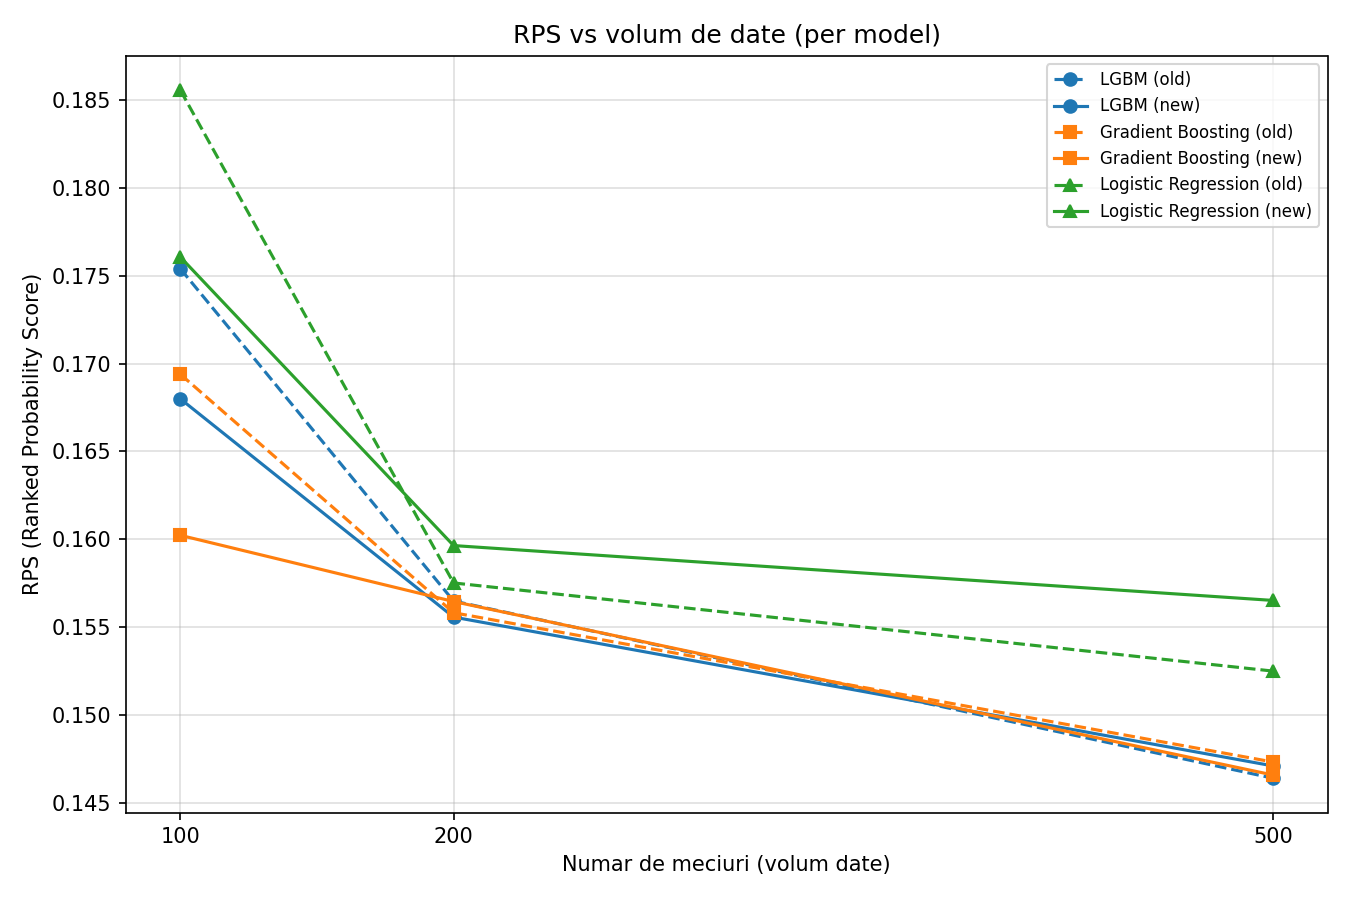
\includegraphics[width=\textwidth]{figures/rps_vs_matches.png}
    \caption{RPS în funcție de volumul de date}
    \label{fig:rps_vs_matches}
\end{subfigure}
\hfill
\begin{subfigure}{0.48\textwidth}
    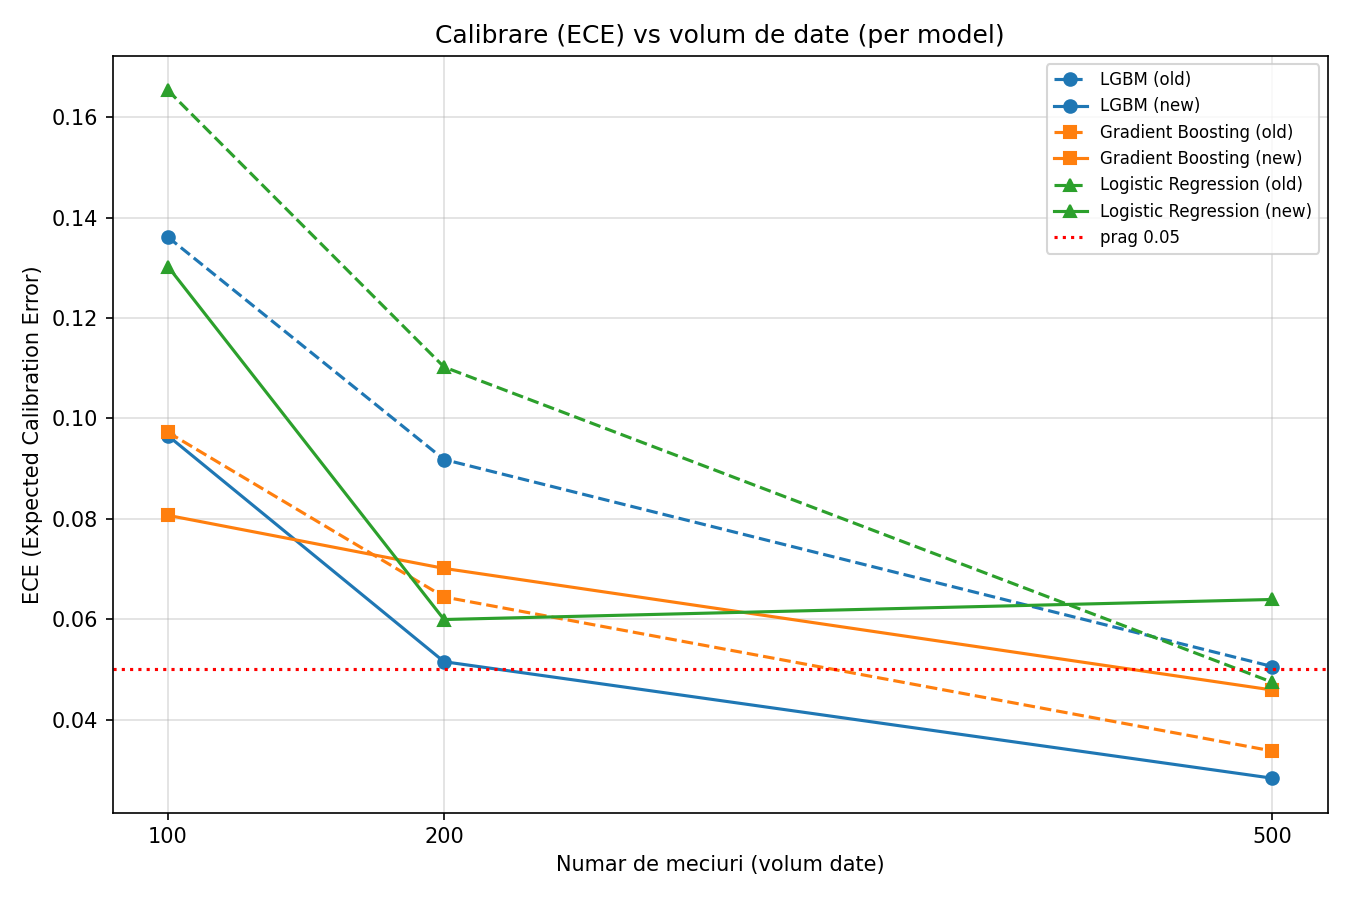
\includegraphics[width=\textwidth]{figures/calibration_vs_matches.png}
    \caption{ECE în funcție de volumul de date}
    \label{fig:calib_vs_matches}
\end{subfigure}
\caption{Evoluția metricilor probabilistice la scalarea volumului de date.
         Liniile întrerupte reprezintă configurația cu caracteristici de
         bază, iar liniile continue configurația cu caracteristici extinse.
         Linia orizontală punctată la ECE = 0.05 marchează pragul de
         acceptabilitate pentru uz tactic \cite{Robberechts2019}.}
\label{fig:scalare_metrici}
\end{figure}

Toate modelele își îmbunătățesc consistent metricile pe măsură ce volumul
crește. Saltul de la 100 la 200 de meciuri este cel mai pronunțat; de
exemplu, pentru caracteristici extinse, ECE al LightGBM scade de la 0.097
la 0.052, traversând pragul de 0.05. Trecerea la 500 de meciuri aduce
câștiguri mai mici, dar consolidează avantajul modelelor de ansamblu
(Gradient Boosting și LightGBM) față de Regresia Logistică. În contextul
aplicației, acest comportament este relevant deoarece arată că un volum
moderat de date (în jur de 500 de meciuri) este suficient pentru a obține
probabilități bine calibrate, fapt care reduce costul de reantrenare atunci
când se dorește actualizarea modelului cu date noi.

\subsection{Impactul caracteristicilor derivate}

Tabelul~\ref{tab:scalare_full} permite și compararea directă a celor două
seturi de caracteristici la volum fix de 500 de meciuri, izolând astfel
efectul celor 9 caracteristici derivate. Rezultatele relevă un tipar
interesant. LightGBM obține cele mai bune valori de log-loss și RPS pe
setul de bază (0.774, respectiv 0.146), dar cea mai bună calibrare pe setul
extins (ECE = 0.028, cea mai mică valoare dintre toate cele 18
configurații). Gradient Boosting are o calibrare mai bună pe setul de bază
(ECE = 0.034) decât pe cel extins (0.046). Regresia Logistică este singurul
model care se degradează consistent prin adăugarea caracteristicilor
derivate: acuratețea scade de la 0.626 la 0.618, iar ECE crește de la 0.047
la 0.064. Acest comportament este așteptat, întrucât ipoteza de liniaritate
a Regresiei Logistice nu poate exploata relațiile non-liniare introduse de
caracteristicile de momentum și de context temporal.

\begin{figure}[H]
\centering
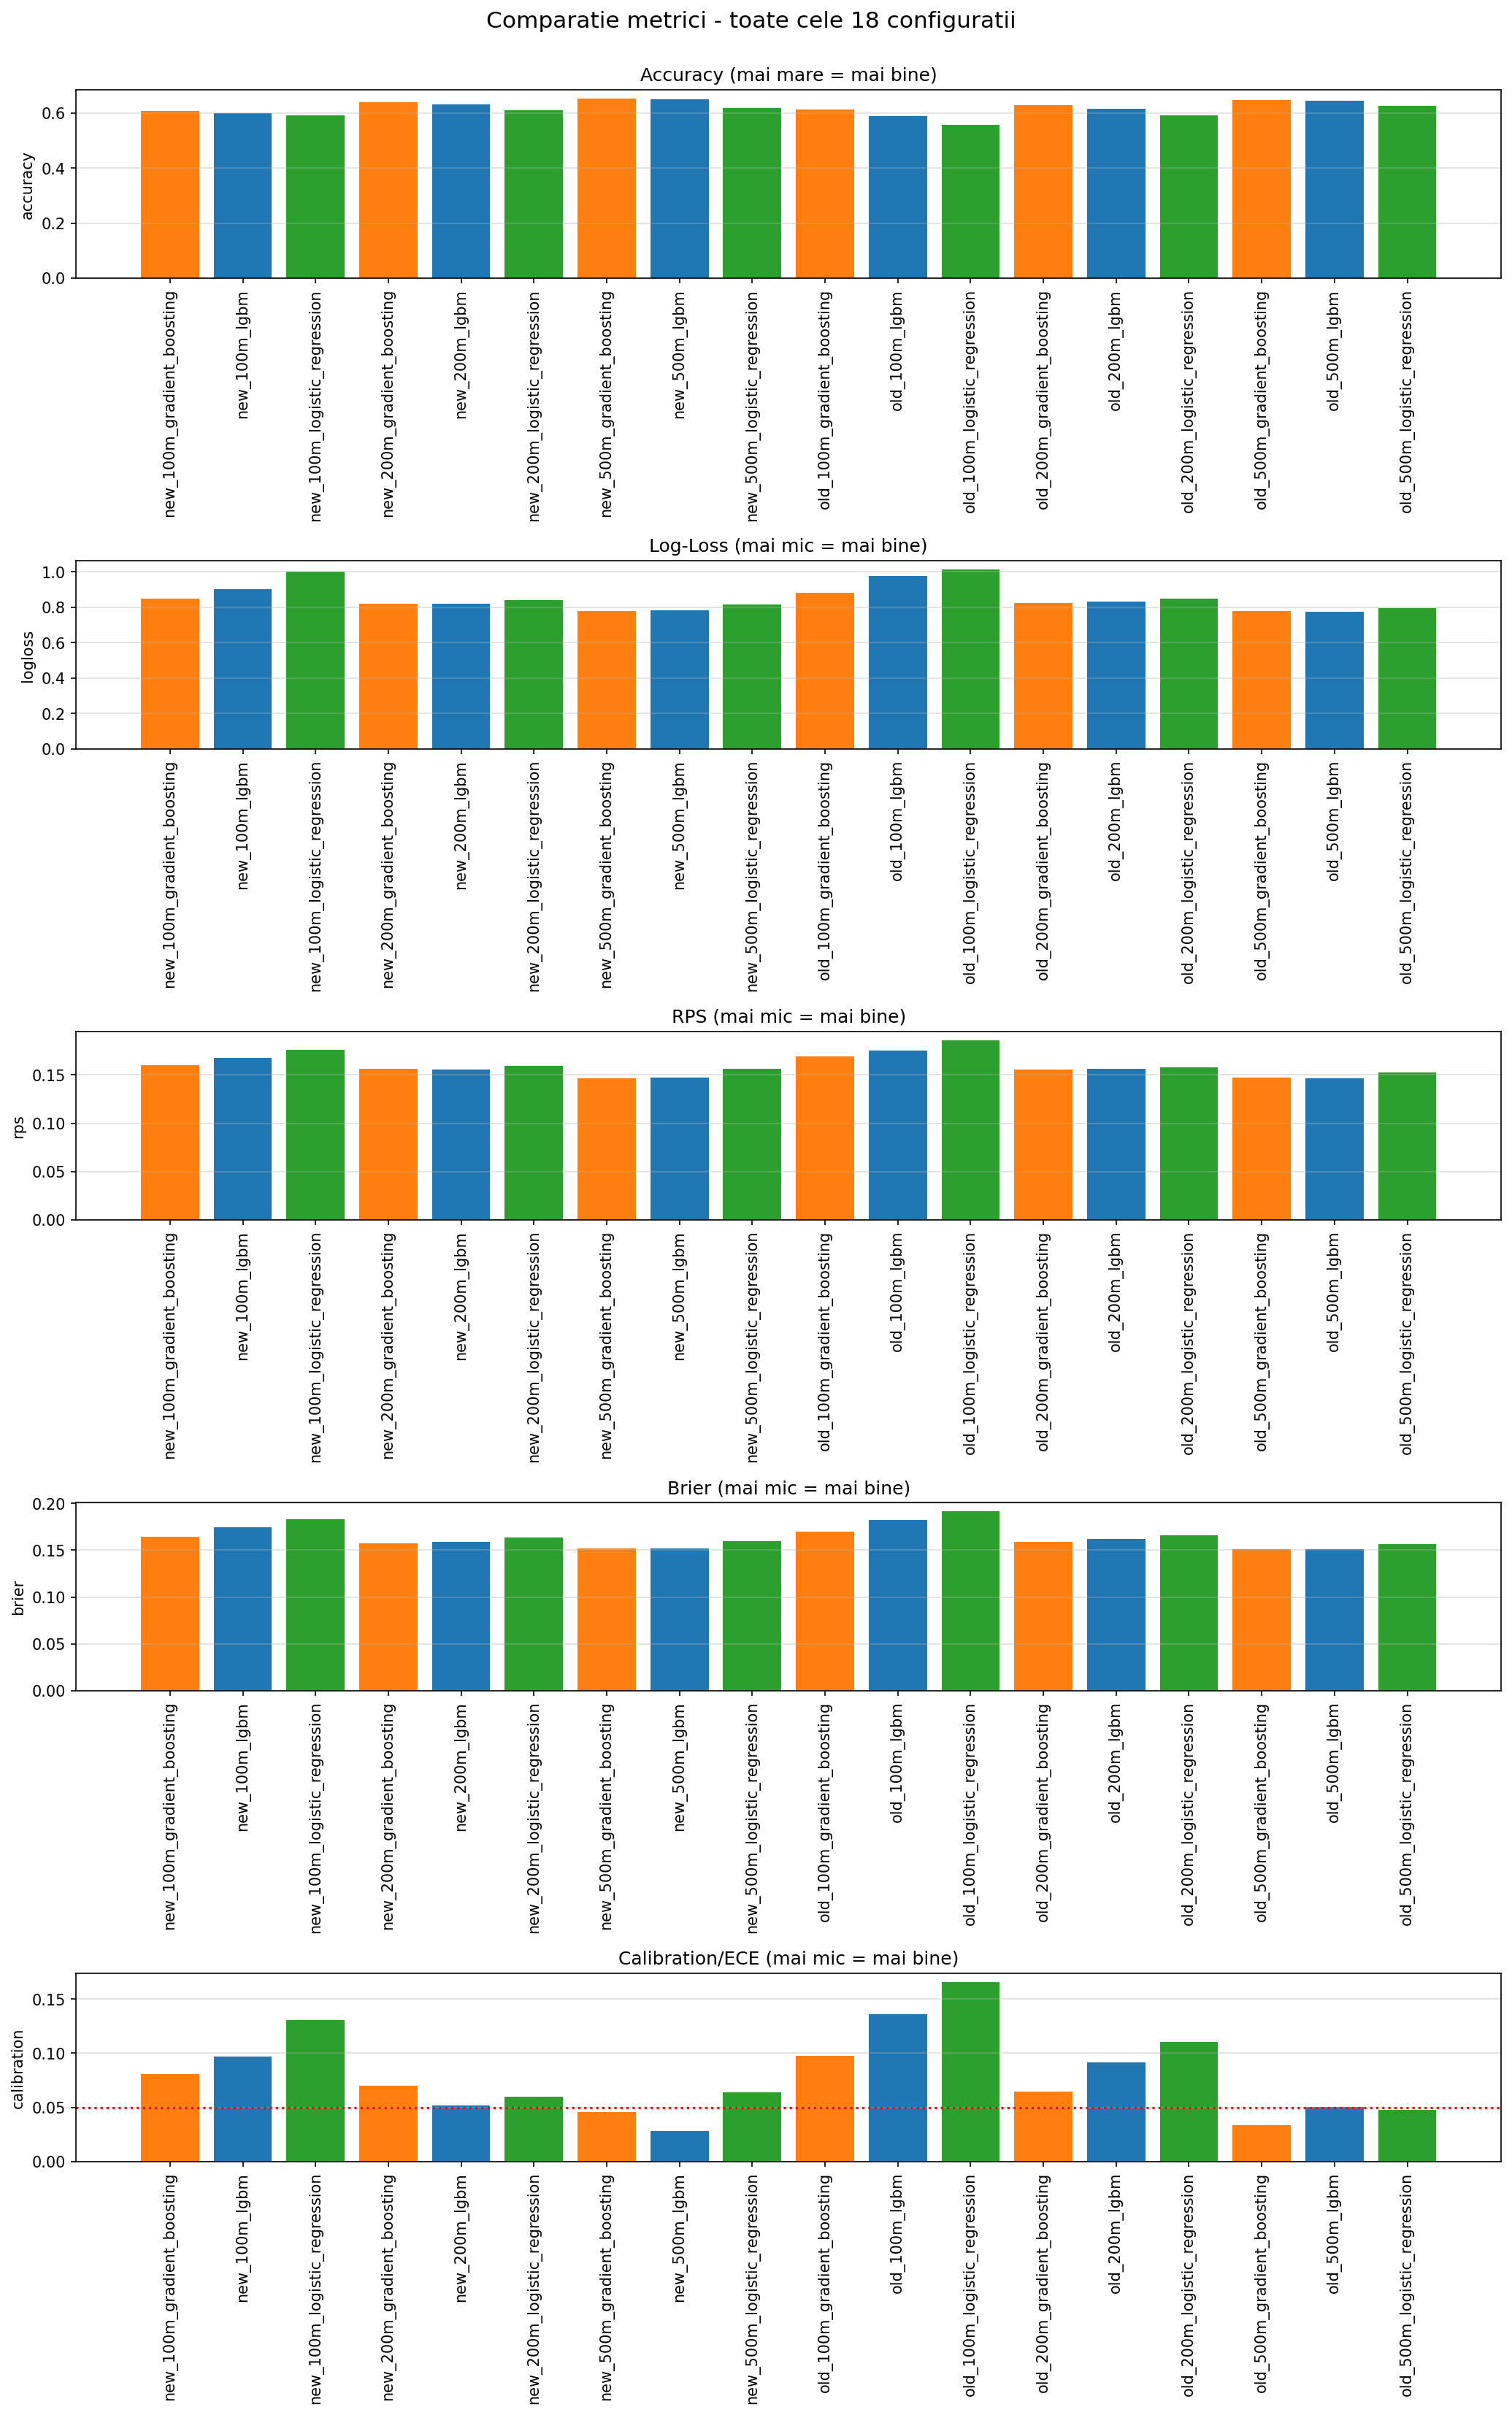
\includegraphics[width=0.85\textwidth]{figures/comparatie_metrici_500.png}
\caption{Comparație completă a celor 6 configurații la 500 de meciuri
         (3 modele $\times$ 2 seturi de caracteristici) pe toate cele cinci
         metrici. Fiecare grup de bare reprezintă o metrică, iar în cadrul
         fiecărui grup barele corespund celor 6 combinații.}
\label{fig:comparatie_completa}
\end{figure}

% ----------------------------------------------------------------
\section{Selecția Modelului Final}
\label{sec:selectie_model}

Pe baza rezultatelor obținute la 500 de meciuri, modelul ales pentru
integrarea în aplicație este \textbf{LightGBM antrenat cu caracteristici
extinse} (configurația \texttt{LGBM-new-500}). Decizia s-a bazat în primul
rând pe calibrare, metrica cea mai relevantă pentru o aplicație care
afișează probabilități de câștig, și în al doilea rând pe eficiența
computațională.

Argumentul de calibrare este decisiv. Configurația \texttt{LGBM-new-500}
obține un ECE de 0.028, cea mai mică valoare dintre toate cele 18
configurații evaluate, cu aproximativ 38\% mai bună decât cea a
configurației \texttt{GB-new-500} (ECE = 0.046). Într-o aplicație care
afișează probabilități de câștig (Home Win, Draw, Away Win), calibrarea
este metrica definitorie: o probabilitate de 70\% afișată utilizatorului
trebuie să corespundă unei frecvențe reale de aproximativ 70\%, nu doar să
clasifice corect favorita.

Pe celelalte metrici, cele două modele de ansamblu sunt practic
echivalente la 500 de meciuri. Pe RPS și Brier Score, \texttt{LGBM-new-500}
și \texttt{GB-new-500} obțin valori identice (RPS = 0.147, BS = 0.152), iar
diferența de acuratețe este de doar 0.003 (0.649 față de 0.652). În
schimb, eficiența computațională diferă substanțial: o serie completă de
antrenare LightGBM la 500 de meciuri s-a încheiat în aproximativ 10 minute,
față de peste 17 ore pentru Gradient Boosting pe același set cu
caracteristici extinse, un raport de ordinul 100:1 care face din LightGBM
singurul model practic pentru reantrenare periodică pe volume crescânde de
date.

Tabelul~\ref{tab:selectie_finala} rezumă comparația directă dintre cele
două modele candidate la 500 de meciuri cu caracteristici extinse.

\begin{table}[htbp]
\centering
\begin{tabular}{|l|ccccc|c|}
\hline
\textbf{Model} & \textbf{Acc} & \textbf{LL} & \textbf{RPS}
& \textbf{BS} & \textbf{ECE} & \textbf{Timp antrenare} \\
\hline
Gradient Boosting & \textbf{0.652} & 0.781 & 0.147 & 0.152 & 0.046
& $\sim$17 h \\
LightGBM          & 0.649 & 0.782 & 0.147 & 0.152 & \textbf{0.028}
& $\sim$10 min \\
\hline
\end{tabular}
\caption{Comparație directă între modelele candidate la selecția finală
         (500 de meciuri, caracteristici extinse). LightGBM este ales pe
         baza calibrării superioare (singura diferență semnificativă între
         cele două modele) și a eficienței computaționale, cu pierdere
         neglijabilă pe celelalte metrici.}
\label{tab:selectie_finala}
\end{table}

Pe baza acestei decizii, modelul final LightGBM a fost reantrenat pe
întregul set de antrenare (cele 2.771 de meciuri) cu configurația optimă
de hiperparametri din Tabelul~\ref{tab:hyperparams} și serializat ca
\texttt{lgbm\_final\_model.pkl} pentru integrarea în backend. Evaluat pe
setul de test comun, modelul final obține o acuratețe de 65.7\%, un RPS de
0.1431, un Brier Score de 0.1472 și un ECE de 0.0309. Este important de
remarcat distincția dintre valoarea de calibrare obținută în experimentul
pe 500 de meciuri (ECE = 0.028) și cea a modelului final (ECE = 0.0309):
prima caracterizează configurația de experimentare, în timp ce a doua
caracterizează modelul efectiv integrat în aplicație, antrenat pe toate
cele 2.771 de meciuri de antrenare. Ambele valori se situează sub pragul
de 0.05 considerat acceptabil pentru uz tactic în literatura de
specialitate \cite{Robberechts2019}.

% ----------------------------------------------------------------
\section{Identificarea Momentelor Decisive}

Pe lângă estimarea probabilităților, sistemul detectează automat
evenimentele care au influențat cel mai mult deznodământul partidei, pe
baza conceptului de \textit{Win Probability Added} (WPA) introdus de Tango
et al. \cite{Tango2007} și aplicat în timp real de Burke \cite{Burke2010}.
Ideea fundamentală este de a cuantifica impactul fiecărui eveniment prin
variația de probabilitate pe care o produce: pentru două snapshots
consecutive, se calculează diferența dintre probabilitatea de victorie
estimată după eveniment și cea estimată înainte de eveniment. Un eveniment
cu o variație mare reprezintă un moment în care soarta meciului s-a
schimbat semnificativ.

Concret, după ce modelul produce traiectoria probabilistică a meciului,
sistemul parcurge succesiv momentele și reține drept decisive doar
evenimentele care produc o variație a probabilității mai mare de 5\% față
de momentul anterior. Pragul de 5\% a fost ales empiric pentru a filtra
fluctuațiile minore și a păstra doar evenimentele cu impact real asupra
dinamicii meciului. Exemplele tipice de momente decisive detectate sunt
golurile, care produc de regulă o creștere de ordinul a 15 puncte
procentuale a probabilității echipei care marchează, cartonașele roșii,
care produc o scădere de ordinul a 10 puncte procentuale pentru echipa
sancționată, precum și creșterile susținute de presiune din minutele
finale. Pentru fiecare moment decisiv, sistemul reține minutul,
probabilitățile înainte și după eveniment, precum și jucătorul implicat,
informații utilizate ulterior în interfața aplicației pentru a construi o
naratologie cantitativă a partidei.

% ----------------------------------------------------------------
\section{Discuția rezultatelor}
\label{sec:discutie}

Modelul final, LightGBM cu caracteristici extinse antrenat pe cele 2.771
de meciuri, obține pe setul de test o acuratețe de 65.7\%, un RPS de
0.1431, un Brier Score de 0.1472 și un ECE de 0.0309, valori competitive
față de literatura de specialitate \cite{Robberechts2019}. Valoarea ECE de
0.0309 se situează semnificativ sub pragul de 0.05 considerat acceptabil
pentru uz tactic, ceea ce înseamnă că probabilitățile afișate utilizatorului
reflectă fidel frecvențele reale: dacă modelul estimează 70\% pentru
victoria gazdei, echipa respectivă câștigă în aproximativ
$70\% \pm 3.09\%$ din situațiile similare.

Experimentele comparative conduc la trei concluzii clare. Prima este că
volumul de date reprezintă factorul dominant: fiecare metrică se
îmbunătățește consistent pentru toate modelele pe măsura creșterii datelor
de antrenare, saltul de la 100 la 200 de meciuri fiind cel mai pronunțat
(ECE al LightGBM scade de la 0.097 la 0.052, traversând pragul de 0.05),
iar trecerea la 500 de meciuri consolidând aceste câștiguri cu o rată de
îmbunătățire mai mică, ceea ce sugerează convergența spre un nivel stabil
de performanță.

A doua concluzie este că adăugarea caracteristicilor derivate îmbunătățește
calibrarea LightGBM, dar nu și pe cea a celorlalte modele. Cele 9
caracteristici de momentum și context reduc ECE al LightGBM de la 0.051
(set de bază, 500 de meciuri) la 0.028 (set extins, 500 de meciuri).
Regresia Logistică, în schimb, se degradează prin adăugarea acestor
caracteristici (ECE crește de la 0.047 la 0.064 la 500 de meciuri), ceea ce
confirmă că un model liniar nu poate exploata relațiile non-liniare
introduse.

A treia concluzie este că modelele de ansamblu domină Regresia Logistică,
cu diferențe mici între ele. La 500 de meciuri cu caracteristici extinse,
Gradient Boosting și LightGBM obțin valori practic identice pe RPS (0.147)
și Brier Score (0.152), diferența de acuratețe fiind de doar 0.003.
Regresia Logistică rămâne constant inferioară la orice volum și pe orice
metrică, ceea ce confirmă că non-liniaritatea capturată de modelele de
ansamblu este necesară pentru această problemă.
